\documentclass[twoside]{book}

% Packages required by doxygen
\usepackage{fixltx2e}
\usepackage{calc}
\usepackage{doxygen}
\usepackage[export]{adjustbox} % also loads graphicx
\usepackage{graphicx}
\usepackage[utf8]{inputenc}
\usepackage{makeidx}
\usepackage{multicol}
\usepackage{multirow}
\PassOptionsToPackage{warn}{textcomp}
\usepackage{textcomp}
\usepackage[nointegrals]{wasysym}
\usepackage[table]{xcolor}

% Font selection
\usepackage[T1]{fontenc}
\usepackage[scaled=.90]{helvet}
\usepackage{courier}
\usepackage{amssymb}
\usepackage{sectsty}
\renewcommand{\familydefault}{\sfdefault}
\allsectionsfont{%
  \fontseries{bc}\selectfont%
  \color{darkgray}%
}
\renewcommand{\DoxyLabelFont}{%
  \fontseries{bc}\selectfont%
  \color{darkgray}%
}
\newcommand{\+}{\discretionary{\mbox{\scriptsize$\hookleftarrow$}}{}{}}

% Page & text layout
\usepackage{geometry}
\geometry{%
  a4paper,%
  top=2.5cm,%
  bottom=2.5cm,%
  left=2.5cm,%
  right=2.5cm%
}
\tolerance=750
\hfuzz=15pt
\hbadness=750
\setlength{\emergencystretch}{15pt}
\setlength{\parindent}{0cm}
\setlength{\parskip}{3ex plus 2ex minus 2ex}
\makeatletter
\renewcommand{\paragraph}{%
  \@startsection{paragraph}{4}{0ex}{-1.0ex}{1.0ex}{%
    \normalfont\normalsize\bfseries\SS@parafont%
  }%
}
\renewcommand{\subparagraph}{%
  \@startsection{subparagraph}{5}{0ex}{-1.0ex}{1.0ex}{%
    \normalfont\normalsize\bfseries\SS@subparafont%
  }%
}
\makeatother

% Headers & footers
\usepackage{fancyhdr}
\pagestyle{fancyplain}
\fancyhead[LE]{\fancyplain{}{\bfseries\thepage}}
\fancyhead[CE]{\fancyplain{}{}}
\fancyhead[RE]{\fancyplain{}{\bfseries\leftmark}}
\fancyhead[LO]{\fancyplain{}{\bfseries\rightmark}}
\fancyhead[CO]{\fancyplain{}{}}
\fancyhead[RO]{\fancyplain{}{\bfseries\thepage}}
\fancyfoot[LE]{\fancyplain{}{}}
\fancyfoot[CE]{\fancyplain{}{}}
\fancyfoot[RE]{\fancyplain{}{\bfseries\scriptsize Generated by Doxygen }}
\fancyfoot[LO]{\fancyplain{}{\bfseries\scriptsize Generated by Doxygen }}
\fancyfoot[CO]{\fancyplain{}{}}
\fancyfoot[RO]{\fancyplain{}{}}
\renewcommand{\footrulewidth}{0.4pt}
\renewcommand{\chaptermark}[1]{%
  \markboth{#1}{}%
}
\renewcommand{\sectionmark}[1]{%
  \markright{\thesection\ #1}%
}

% Indices & bibliography
\usepackage{natbib}
\usepackage[titles]{tocloft}
\setcounter{tocdepth}{3}
\setcounter{secnumdepth}{5}
\makeindex

% Hyperlinks (required, but should be loaded last)
\usepackage{ifpdf}
\ifpdf
  \usepackage[pdftex,pagebackref=true]{hyperref}
\else
  \usepackage[ps2pdf,pagebackref=true]{hyperref}
\fi
\hypersetup{%
  colorlinks=true,%
  linkcolor=blue,%
  citecolor=blue,%
  unicode%
}

% Custom commands
\newcommand{\clearemptydoublepage}{%
  \newpage{\pagestyle{empty}\cleardoublepage}%
}

\usepackage{caption}
\captionsetup{labelsep=space,justification=centering,font={bf},singlelinecheck=off,skip=4pt,position=top}

%===== C O N T E N T S =====

\begin{document}

% Titlepage & ToC
\hypersetup{pageanchor=false,
             bookmarksnumbered=true,
             pdfencoding=unicode
            }
\pagenumbering{roman}
\begin{titlepage}
\vspace*{7cm}
\begin{center}%
{\Large L\+O53\+\_\+\+Android }\\
\vspace*{1cm}
{\large Generated by Doxygen 1.8.11}\\
\end{center}
\end{titlepage}
\clearemptydoublepage
\tableofcontents
\clearemptydoublepage
\pagenumbering{arabic}
\hypersetup{pageanchor=true}

%--- Begin generated contents ---
\chapter{Hierarchical Index}
\section{Class Hierarchy}
This inheritance list is sorted roughly, but not completely, alphabetically\+:\begin{DoxyCompactList}
\item \contentsline{section}{com.\+servlet.\+utilities.\+Fingerprint}{\pageref{classcom_1_1servlet_1_1utilities_1_1_fingerprint}}{}
\item \contentsline{section}{com.\+servlet.\+utilities.\+Location}{\pageref{classcom_1_1servlet_1_1utilities_1_1_location}}{}
\item \contentsline{section}{com.\+servlet.\+utilities.\+Query\+With\+Context}{\pageref{classcom_1_1servlet_1_1utilities_1_1_query_with_context}}{}
\item \contentsline{section}{com.\+servlet.\+utilities.\+Rssi\+Sample}{\pageref{classcom_1_1servlet_1_1utilities_1_1_rssi_sample}}{}
\item \contentsline{section}{com.\+servlet.\+utilities.\+Url\+Address}{\pageref{enumcom_1_1servlet_1_1utilities_1_1_url_address}}{}
\item Http\+Servlet\begin{DoxyCompactList}
\item \contentsline{section}{com.\+servlet.\+calibration.\+Calibration\+Servlet}{\pageref{classcom_1_1servlet_1_1calibration_1_1_calibration_servlet}}{}
\item \contentsline{section}{com.\+servlet.\+debug.\+Debug\+Servlet}{\pageref{classcom_1_1servlet_1_1debug_1_1_debug_servlet}}{}
\item \contentsline{section}{com.\+servlet.\+positioning.\+Positioning\+Servlet}{\pageref{classcom_1_1servlet_1_1positioning_1_1_positioning_servlet}}{}
\end{DoxyCompactList}
\end{DoxyCompactList}

\chapter{Class Index}
\section{Class List}
Here are the classes, structs, unions and interfaces with brief descriptions\+:\begin{DoxyCompactList}
\item\contentsline{section}{\hyperlink{classjwabo_1_1lo53__project_1_1_calibrate_activity}{jwabo.\+lo53\+\_\+project.\+Calibrate\+Activity} }{\pageref{classjwabo_1_1lo53__project_1_1_calibrate_activity}}{}
\item\contentsline{section}{\hyperlink{classjwabo_1_1lo53__project_1_1_locate_activity}{jwabo.\+lo53\+\_\+project.\+Locate\+Activity} }{\pageref{classjwabo_1_1lo53__project_1_1_locate_activity}}{}
\item\contentsline{section}{\hyperlink{classjwabo_1_1lo53__project_1_1_main_activity}{jwabo.\+lo53\+\_\+project.\+Main\+Activity} }{\pageref{classjwabo_1_1lo53__project_1_1_main_activity}}{}
\item\contentsline{section}{\hyperlink{classjwabo_1_1lo53__project_1_1_settings_activity}{jwabo.\+lo53\+\_\+project.\+Settings\+Activity} }{\pageref{classjwabo_1_1lo53__project_1_1_settings_activity}}{}
\end{DoxyCompactList}

\chapter{Class Documentation}
\hypertarget{classjwabo_1_1lo53__project_1_1_calibrate_activity}{}\section{jwabo.\+lo53\+\_\+project.\+Calibrate\+Activity Class Reference}
\label{classjwabo_1_1lo53__project_1_1_calibrate_activity}\index{jwabo.\+lo53\+\_\+project.\+Calibrate\+Activity@{jwabo.\+lo53\+\_\+project.\+Calibrate\+Activity}}
Inheritance diagram for jwabo.\+lo53\+\_\+project.\+Calibrate\+Activity\+:\begin{figure}[H]
\begin{center}
\leavevmode
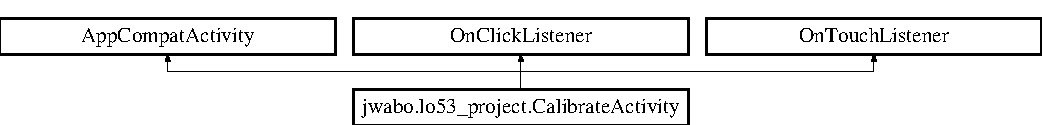
\includegraphics[height=1.666667cm]{classjwabo_1_1lo53__project_1_1_calibrate_activity}
\end{center}
\end{figure}
\subsection*{Public Member Functions}
\begin{DoxyCompactItemize}
\item 
void \hyperlink{classjwabo_1_1lo53__project_1_1_calibrate_activity_adfec3fba76931e7d6081486441207535}{on\+Create} (Bundle saved\+Instance\+State)
\item 
void {\bfseries on\+Click} (View view)\hypertarget{classjwabo_1_1lo53__project_1_1_calibrate_activity_ac579359bd471e55501bfe0ab39453548}{}\label{classjwabo_1_1lo53__project_1_1_calibrate_activity_ac579359bd471e55501bfe0ab39453548}

\item 
boolean {\bfseries on\+Touch} (View view, Motion\+Event motion\+Event)\hypertarget{classjwabo_1_1lo53__project_1_1_calibrate_activity_a18c4b7134a6901af9633258b521381c1}{}\label{classjwabo_1_1lo53__project_1_1_calibrate_activity_a18c4b7134a6901af9633258b521381c1}

\end{DoxyCompactItemize}


\subsection{Detailed Description}
Activity \hyperlink{classjwabo_1_1lo53__project_1_1_calibrate_activity}{Calibrate\+Activity} used for calibrating the positioning system 

\subsection{Member Function Documentation}
\index{jwabo\+::lo53\+\_\+project\+::\+Calibrate\+Activity@{jwabo\+::lo53\+\_\+project\+::\+Calibrate\+Activity}!on\+Create@{on\+Create}}
\index{on\+Create@{on\+Create}!jwabo\+::lo53\+\_\+project\+::\+Calibrate\+Activity@{jwabo\+::lo53\+\_\+project\+::\+Calibrate\+Activity}}
\subsubsection[{\texorpdfstring{on\+Create(\+Bundle saved\+Instance\+State)}{onCreate(Bundle savedInstanceState)}}]{\setlength{\rightskip}{0pt plus 5cm}void jwabo.\+lo53\+\_\+project.\+Calibrate\+Activity.\+on\+Create (
\begin{DoxyParamCaption}
\item[{Bundle}]{saved\+Instance\+State}
\end{DoxyParamCaption}
)}\hypertarget{classjwabo_1_1lo53__project_1_1_calibrate_activity_adfec3fba76931e7d6081486441207535}{}\label{classjwabo_1_1lo53__project_1_1_calibrate_activity_adfec3fba76931e7d6081486441207535}
Called when the activity is first created. 

The documentation for this class was generated from the following file\+:\begin{DoxyCompactItemize}
\item 
app/src/main/java/jwabo/lo53\+\_\+project/Calibrate\+Activity.\+java\end{DoxyCompactItemize}

\hypertarget{classjwabo_1_1lo53__project_1_1_locate_activity}{}\section{jwabo.\+lo53\+\_\+project.\+Locate\+Activity Class Reference}
\label{classjwabo_1_1lo53__project_1_1_locate_activity}\index{jwabo.\+lo53\+\_\+project.\+Locate\+Activity@{jwabo.\+lo53\+\_\+project.\+Locate\+Activity}}
Inheritance diagram for jwabo.\+lo53\+\_\+project.\+Locate\+Activity\+:\begin{figure}[H]
\begin{center}
\leavevmode
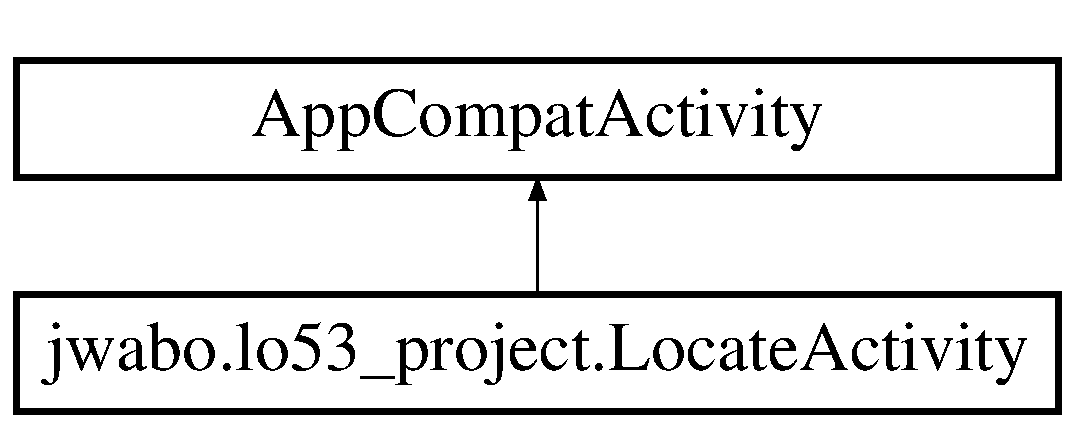
\includegraphics[height=2.000000cm]{classjwabo_1_1lo53__project_1_1_locate_activity}
\end{center}
\end{figure}
\subsection*{Protected Member Functions}
\begin{DoxyCompactItemize}
\item 
void {\bfseries on\+Create} (Bundle saved\+Instance\+State)\hypertarget{classjwabo_1_1lo53__project_1_1_locate_activity_a35e58fdd95af4ca7dd8b0f29ecdb3539}{}\label{classjwabo_1_1lo53__project_1_1_locate_activity_a35e58fdd95af4ca7dd8b0f29ecdb3539}

\end{DoxyCompactItemize}


\subsection{Detailed Description}
Activity \hyperlink{classjwabo_1_1lo53__project_1_1_locate_activity}{Locate\+Activity} used for locating the current mobile device 

The documentation for this class was generated from the following file\+:\begin{DoxyCompactItemize}
\item 
app/src/main/java/jwabo/lo53\+\_\+project/Locate\+Activity.\+java\end{DoxyCompactItemize}

\hypertarget{classjwabo_1_1lo53__project_1_1_main_activity}{}\section{jwabo.\+lo53\+\_\+project.\+Main\+Activity Class Reference}
\label{classjwabo_1_1lo53__project_1_1_main_activity}\index{jwabo.\+lo53\+\_\+project.\+Main\+Activity@{jwabo.\+lo53\+\_\+project.\+Main\+Activity}}
Inheritance diagram for jwabo.\+lo53\+\_\+project.\+Main\+Activity\+:\begin{figure}[H]
\begin{center}
\leavevmode
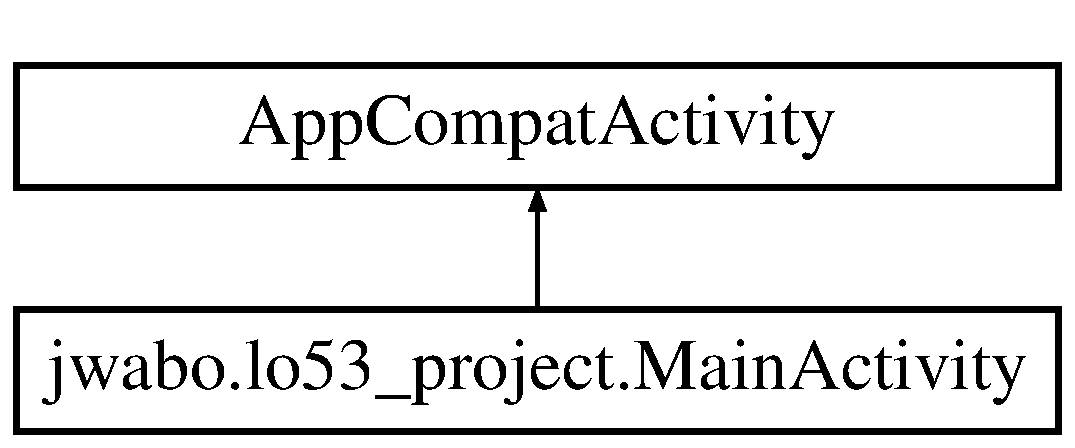
\includegraphics[height=2.000000cm]{classjwabo_1_1lo53__project_1_1_main_activity}
\end{center}
\end{figure}
\subsection*{Protected Member Functions}
\begin{DoxyCompactItemize}
\item 
void {\bfseries on\+Create} (Bundle saved\+Instance\+State)\hypertarget{classjwabo_1_1lo53__project_1_1_main_activity_ac9fde4f7b8610d56e2b8cbb2fc4bcfa9}{}\label{classjwabo_1_1lo53__project_1_1_main_activity_ac9fde4f7b8610d56e2b8cbb2fc4bcfa9}

\end{DoxyCompactItemize}


\subsection{Detailed Description}
Activity \hyperlink{classjwabo_1_1lo53__project_1_1_main_activity}{Main\+Activity} 

The documentation for this class was generated from the following file\+:\begin{DoxyCompactItemize}
\item 
app/src/main/java/jwabo/lo53\+\_\+project/Main\+Activity.\+java\end{DoxyCompactItemize}

\hypertarget{classjwabo_1_1lo53__project_1_1_settings_activity}{}\section{jwabo.\+lo53\+\_\+project.\+Settings\+Activity Class Reference}
\label{classjwabo_1_1lo53__project_1_1_settings_activity}\index{jwabo.\+lo53\+\_\+project.\+Settings\+Activity@{jwabo.\+lo53\+\_\+project.\+Settings\+Activity}}
Inheritance diagram for jwabo.\+lo53\+\_\+project.\+Settings\+Activity\+:\begin{figure}[H]
\begin{center}
\leavevmode
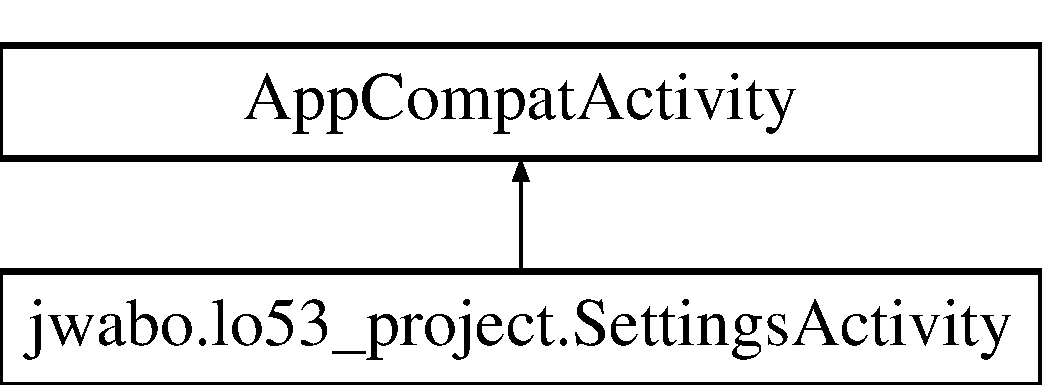
\includegraphics[height=2.000000cm]{classjwabo_1_1lo53__project_1_1_settings_activity}
\end{center}
\end{figure}
\subsection*{Protected Member Functions}
\begin{DoxyCompactItemize}
\item 
void {\bfseries on\+Create} (Bundle saved\+Instance\+State)\hypertarget{classjwabo_1_1lo53__project_1_1_settings_activity_ae221b0e510188aa06fd01b18b5de6cfa}{}\label{classjwabo_1_1lo53__project_1_1_settings_activity_ae221b0e510188aa06fd01b18b5de6cfa}

\end{DoxyCompactItemize}


\subsection{Detailed Description}
Activity \hyperlink{classjwabo_1_1lo53__project_1_1_settings_activity}{Settings\+Activity} used for setting the address of the servlet and the port 

The documentation for this class was generated from the following file\+:\begin{DoxyCompactItemize}
\item 
app/src/main/java/jwabo/lo53\+\_\+project/Settings\+Activity.\+java\end{DoxyCompactItemize}

%--- End generated contents ---

% Index
\backmatter
\newpage
\phantomsection
\clearemptydoublepage
\addcontentsline{toc}{chapter}{Index}
\printindex

\end{document}
